%% LyX 2.1.3 created this file.  For more info, see http://www.lyx.org/.
%% Do not edit unless you really know what you are doing.
\documentclass[oneside,english]{amsart}
\usepackage[T1]{fontenc}
\usepackage[latin9]{inputenc}
\usepackage{geometry}
\geometry{verbose,tmargin=1cm,bmargin=1cm,lmargin=1cm,rmargin=1cm,headheight=1cm,headsep=1cm,footskip=1cm}
\usepackage{mathtools}
\usepackage{amsthm}
\usepackage{amsbsy}
\usepackage{amstext}
\usepackage{amssymb}
\usepackage{graphicx}
\usepackage{esint}

\makeatletter
%%%%%%%%%%%%%%%%%%%%%%%%%%%%%% Textclass specific LaTeX commands.
\numberwithin{equation}{section}
\numberwithin{figure}{section}
\theoremstyle{plain}
\newtheorem{thm}{\protect\theoremname}
  \theoremstyle{definition}
  \newtheorem{defn}[thm]{\protect\definitionname}
 \theoremstyle{definition}
 \newtheorem*{defn*}{\protect\definitionname}
  \theoremstyle{plain}
  \newtheorem{cor}[thm]{\protect\corollaryname}
  \theoremstyle{definition}
  \newtheorem{example}[thm]{\protect\examplename}

\makeatother

\usepackage{babel}
  \providecommand{\corollaryname}{Corollary}
  \providecommand{\definitionname}{Definition}
  \providecommand{\examplename}{Example}
\providecommand{\theoremname}{Theorem}

\begin{document}

\title{Stochastic Processes, SDEs, and Option Pricing}

\maketitle

\section{Measure Theory in 5 Minutes}
\begin{defn}
$\Omega$ is a set called the sample/event space. A $\sigma$-algebra
$\mathcal{F}$ is a family $\mathcal{F}$ of subsets of $\Omega$
with the following properties
\begin{enumerate}
\item $\emptyset\in\mathcal{F}$
\item $F\in\mathcal{F}\Rightarrow F^{C}\in\mathcal{F}$ i.e. $\mathcal{F}$
is closed under complementation.
\item $A_{i}\in\mathcal{F}\Rightarrow\bigcup_{i=1}^{\infty}A_{i}\in\mathcal{F}$
i.e. $\mathcal{F}$ is closed under countable unions.
\end{enumerate}
\end{defn}

\begin{defn}
The pair $\left(\Omega,\mathcal{F}\right)$ is called a measurable
space and the subsets $F$ of $\Omega$ which belond to $\mathcal{F}$
are called $\mathcal{F}$-measurable sets.
\end{defn}

\begin{defn}
A \emph{measure }is a function function $\mu:\mathcal{F}\rightarrow\mathbb{R}_{+}$
such that $\mu\left(\emptyset\right)=0$ and $\mu$ is countably additive
\[
\mu\left(\bigcup_{i=1}^{\infty}E_{i}\right)=\sum_{i=1}^{\infty}E_{i}
\]
 . It ``weighs'' sets. The triple $\left(\Omega,\mathcal{F},\mu\right)$
is appropriately called a \emph{measure space}. If $\mu\left(\Omega\right)<\infty$
then $\left(\Omega,\mathcal{F},\mu\right)$ is called a \emph{finite-measure
space}. 
\end{defn}

\begin{defn}
Let $\left(\Omega,\mathcal{F},\mu\right)$ and $\left(\Omega',\mathcal{F}',\mu'\right)$
be measure spaces. Then a function $X:\Omega\rightarrow\Omega'$ is
$\mathcal{F}-\mathcal{F}'$-\emph{measurable} if for every $U\in\mathcal{F}'$
\[
X^{-1}\left(U\right)=\left\{ \omega\in\Omega;X\left(\omega\right)\in U\right\} \in\mathcal{F}
\]
I.e. pre-images of measurable sets in the \emph{$\sigma$-algebra}
associated with the codomain are measurable sets in the \emph{$\sigma$-algebra}
associated with the domain. 
\end{defn}


Talk a little about defining the Lebesgue integral in terms of simple
functions and approximating continuous functions by simple functions.
\begin{defn}
The \emph{abstract} \emph{Lebesgue integral} of an $\mathcal{F}-\mathcal{F}'$-measurable
function $X:\Omega\rightarrow\Omega'$ on the set $A\in\mathcal{F}'$
is denoted 
\[
\int_{A}Xd\mu\left(\omega\right)
\]
and roughly corresponds to inverse of the typical understanding of
the Riemann integral: fix a value $X=x$ for $x\in A$, find the inverse
image $X^{-1}\left(x\right)=\left\{ \omega:X\left(\omega\right)=x\right\} $,
and find the measure/mass of that set $\mu\left(X^{-1}\left(x\right)\right)=\mu\left(\left\{ \omega:X\left(\omega\right)=x\right\} \right)$
under the measure on the domain $\sigma$-algebra $\mathcal{F}$,
i.e. $\mu$. The \emph{Lebesgue integral} is an abstract Lebesgue
integral with $\mu=\lambda$ the Lebesgue measure\footnote{The unique translation invariant measure that assigns $\lambda\left(\left[a,b\right)\right)=b-a$.}
on $\mathbb{R}$. 
\end{defn}

\begin{defn}
If $\mu\left(\Omega\right)=1$ then $\left(\Omega,\mathcal{F},\mu\right)$
is called a \emph{probability space} and convention is to write $\mu$
as $P$. Furthermore $P$ should be such that for $A_{i}$ such that
$A_{i}\cap A_{j}=\emptyset$ for $i\neq j$ it's the case that $P\left(\bigcup_{i=1}^{\infty}A_{i}\right)=\sum_{i=1}^{n}P\left(A_{i}\right)$,
called countable additivity.
\end{defn}

\begin{defn}
For $\left(\Omega,\mathcal{F},P\right)$ and $\left(\mathbb{R}^{n},\mathcal{B}^{n}\right)$
a \emph{random variable} is an $\mathcal{F}$-\emph{measurable} function
$X:\Omega\rightarrow\mathbb{R}^{n}$.
\end{defn}
Every random variable induces a probability measure $\mu_{X}$ on
$\mathbb{R}^{n}$, defined by
\[
\mu_{X}\left(A\right)=P\left(X^{-1}\left(A\right)\right)
\]
where $B\in\mathcal{B}^{n}$ and $\mathcal{B}^{n}$ is the $\sigma$-algebra
over $\mathbb{R}^{n}$. $\mu_{X}$ is called the \emph{distribution
}or\emph{ law of $X$. }


\section{Stochastic Processes}
\begin{defn}
A stochastic process is a parameterized collection of random variables
$\left\{ X_{t}\right\} _{t\in T}$ with each $X_{t}$ defined on the
same measure space (probability space) $\left(\Omega,\mathcal{F},P\right)$
and $X_{t}:\Omega\rightarrow\mathbb{R}^{n}$.
\end{defn}
The parameter space for $T$ and the range of $X_{t}$ determine taxonomical
classifiction of the process with each possibly being either continuous
or discrete.

For fixed $t$ it's the case that $X_{t}\left(\omega\right)$ is just
a plain random variable 
\[
X_{t}\left(\omega\right):\Omega\rightarrow\mathbb{R}^{n}
\]
and for fixed $\omega$ it's the case that $X_{\omega}\left(t\right)$
is just a function on $\mathbb{R}^{n}$
\[
X_{\omega}\left(t\right):T\rightarrow\mathbb{R}^{n}
\]
called a \emph{path}. Note that this gives a way to identify a function
with each $\omega\in\Omega$ and therefore we may treat $\Omega$
as a subset of $\tilde{\Omega}\subset\left(\mathbb{R}^{n}\right)^{T}$
the space of \emph{all }functions from $T$ to $\mathbb{R}^{n}$. 
\begin{defn}
The \emph{finite-dimensional distributions} $\left\{ \mu_{t_{1},\dots,t_{k}};k\in\mathbb{N},t_{i}\in T\right\} $
of the process $X=\left\{ X_{t}\right\} _{t\in T}$ are the multidimensional
distributions of the random vectors $\left(X_{t_{1}},\dots,X_{t_{k}}\right)$
for any set $\left\{ t_{1},\dots,t_{k}\right\} $.
\end{defn}
These distributions determine many, but not all (and in some important
cases crucially), properties the process $X$. Conversely given a
family of distributions $\left\{ \mu_{t_{1},\dots,t_{k}};k\in\mathbb{N},t_{i}\in T\right\} $(all
finite product distributions indexed by all finite subsets of $T$)
on $\underbrace{\mathbb{R}^{n}\times\cdots\times\mathbb{R}^{n}}_{k}$
one can construct a stochastic process $X=\left\{ X_{t}\right\} _{t\in T}$
which will have $\left\{ \mu_{t_{1},\dots,t_{k}};k\in\mathbb{N},t_{i}\in T\right\} $
as its finite-dimensional distributions given some ``natural'' consistency
conditions.
\begin{thm}
\label{thm:Kolmogorov's-extension-theorem.}Kolmogorov's extension
theorem. For all finite tuples $\left(t_{1},\dots,t_{k}\right)$ with
$t_{i}\in T$ let $\mu_{t_{1},\dots,t_{k}}$ be the probability measures
defined above. If $\mu_{t_{1},\dots,t_{k}}$ satisfy the consistency
conditions
\begin{enumerate}
\item Invariance under permutation: for all permutations $p$ on $\left\{ 1,2,\dots,k\right\} $
\[
\mu_{p\left(t_{1}\right),\dots,p\left(t_{k}\right)}\left(F_{1}\times\cdots\times F_{k}\right)=\mu_{t_{1},\dots,t_{k}}\left(F_{p^{-1}\left(1\right)}\times\cdots\times F_{p^{-1}\left(k\right)}\right)
\]

\item Invariance under marginalization over probability 1 events: 
\[
\mu_{t_{1},\dots,t_{k}}\left(F_{1}\times\cdots\times F_{k}\right)=\mu_{t_{1},\dots,t_{k},t_{k+1},\dots,t_{k+m}}\left(F_{1}\times\cdots\times F_{k}\times\underbrace{\mathbb{R}^{n}\times\cdots\times\mathbb{R}^{n}}_{m}\right)
\]

\end{enumerate}

then there exists a probability space $\left(\Omega,\mathcal{F},P\right)$
and a stochastic process $X=\left\{ X_{t}\right\} _{t\in T}$ on $\Omega$
with $\mu_{t_{1},\dots,t_{k}}$ as its finite-dimensional distributions.

\end{thm}
Kolmogorov's extension is actually an if and only if: any stochastic
process trivially has these properties. The power of Kolmogorov extension
is that the typical workflow is to define a stochastic process by
its finite-dimensional distributions and that is completely sufficient\footnote{Kolmogorov extension guarnatees there is a correspondent probability
space and process.}.


\section{Brownian Motion}
\begin{defn}
Fix $x\in\mathbb{R}$ and define 
\[
p\left(t,x,y\right)=\frac{1}{\sqrt{2\pi t}}e^{-\frac{\left(x-y\right)^{2}}{2t}}
\]
for $y\in\mathbb{R}$. Then for $0<t_{1}<t_{2}<\cdots<t_{n}$ define
a measure $\mu_{t_{1},\dots,t_{k}}$ on $\mathbb{R}^{k}$ by 
\begin{eqnarray*}
\mu_{t_{1},\dots,t_{k}}\left(F_{1}\times\cdots\times F_{k}\right) & = & \int_{F_{1}}\cdots\int_{F_{k}}p\left(t_{1},x,x_{1}\right)p\left(t_{2}-t_{1},x_{1},x_{2}\right)\cdots\\
 &  & p\left(t_{k}-t_{k-1},x_{k-1},x_{k}\right)dx_{1}dx_{2}\cdots dx_{k}
\end{eqnarray*}
for $F_{i}\subset\mathbb{R}$ with the convention that $p\left(0,x,y\right)dx=\delta_{x}\left(y\right)$
a unit point mass at $x$. Extend to all finite sequences $t_{1},\dots,t_{n}$
and since $\int_{F_{i}}p\left(t,x,y\right)dx=1$ Kolmogorov's Extension
theorem says there exists $\left(\Omega,\mathcal{F},P^{x}\right)$
and a stochastic process $B=\left\{ B_{t}\right\} _{t\geq0}$ on $\Omega$
such that the finite-dimensional distributions of $B_{t}$ are 
\begin{eqnarray}
P^{x}\left(B_{t_{1}}\in F_{1}\times\cdots\times B_{t_{k}}\in F_{k}\right) & = & \int_{F_{1}}\cdots\int_{F_{k}}p\left(t_{1},x,x_{1}\right)p\left(t_{2}-t_{1},x_{1},x_{2}\right)\cdots\label{eq:brownianmotiondef}\\
 &  & p\left(t_{k}-t_{k-1},x_{k-1},x_{k}\right)dx_{1}dx_{2}\cdots dx_{k}\nonumber 
\end{eqnarray}
Such a process\footnote{One that has these finite-dimensional distributions.}
is called a Brownian motion. The paths of a Brownian motion happen
to be almost surely continuous\footnote{Wiener's theorem.} (but nowhere
differentiable!) so with each $\omega\in\Omega$ you can identify
a continuous function $t\rightarrow B_{t}\left(\omega\right)$ from
$\left[0,\infty\right)$ to $\mathbb{R}$. Thus a perspective on Brownian
motion is that it's the space of continuous functions $C\left(\left[0,\infty\right),\mathbb{R}\right)$
equipped with the measures $P^{x}$ above\footnote{Which as discussed are product measures on a function space.}. 
\end{defn}
Here are some of the basic properties of Brownian motion as defined
by defn. \ref{eq:brownianmotiondef}:
\begin{enumerate}
\item Fix the range of $B_{t}$ to be $\mathbb{R}$. For $x=x_{0}$ $B_{t}$
is a \emph{Gaussian process, }i.e. for all $0<t_{1}<t_{2}<\cdots<t_{k}$
the random vector $Z=\left(B_{t_{1}},\dots,B_{t_{k}}\right)\in\left(\mathbb{R}\right)^{k}$
is distributed multinormal. That means there exists a mean vector
$\mathbf{m}\in\left(\mathbb{R}\right)^{k}$ and covariance matrix
$\Sigma=\left[c_{jm}\right]\in\mathbb{R}^{k\times k}$ such that 
\begin{eqnarray*}
E^{x}\left[\exp\left[i\sum_{j=1}^{k}u_{j}B_{t_{j}}\right]\right] & \coloneqq & \int\exp\left[i\sum_{j=1}^{k}u_{j}B_{t_{j}}\right]dP^{x}\\
 & = & \frac{1}{\sqrt[k]{2\pi t_{1}\left(t_{2}-t_{1}\right)\cdots\left(t_{k}-t_{k-1}\right)}}\int_{\mathbb{R}}\cdots\int_{\mathbb{R}}\exp\left[i\sum_{j=1}^{k}u_{j}B_{t_{j}}\right]e^{-\frac{\left(x_{1}-x_{0}\right)^{2}}{2t_{1}}}e^{-\frac{\left(x_{1}-x_{2}\right)^{2}}{2\left(t_{2}-t_{1}\right)}}\cdots\\
 &  & e^{-\frac{\left(x_{k-1}-x_{k}\right)^{2}}{2\left(t_{k}-t_{k-1}\right)}}dx_{1}dx_{2}\cdots dx_{k}
\end{eqnarray*}
Therefore in general\footnote{With $B_{t_{j}}=\mathbf{B}_{t_{j}}\in\mathbb{R}^{n}$}
the finite dimensional distributions of a Brownian motion are multivariate
Gaussians with mean vector $\mathbf{m}=\mathbf{x_{0}}$ and covariance
matrix 
\[
\boldsymbol{\Sigma}=\begin{pmatrix}t_{1}I_{n} & t_{1}I_{n} & \cdots & t_{1}I_{n}\\
t_{1}I_{n} & t_{2}I_{n} & \cdots & t_{2}I_{n}\\
\vdots & \vdots &  & \vdots\\
t_{1}I_{n} & t_{2}I_{n} & \cdots & t_{k}I_{n}
\end{pmatrix}
\]
where $n$ is the dimension of each $B_{t_{j}}$. Therefore, since
each component of a multivariate Gaussian is itself Gaussian with
means and covariances being a function of $\mathbf{m}$ and $\boldsymbol{\Sigma}$
it's the case that 
\[
E^{x}\left[B_{t_{j}}\right]=\mathbf{m}_{t_{j}}=x_{0}
\]
and 
\[
\text{Var}\left(B_{t_{j}}\right)=E^{x}\left[\left(B_{t_{j}}-x_{0}\right)^{2}\right]=t_{j}\text{Tr}\left(I_{n}\right)=nt_{j}
\]
and because of the cascading\footnote{Just think about running your finger down and across the covariance
matrix.} shape of the covariance matrix 
\[
\text{Cov}\left(B_{t_{j}},B_{t_{i}}\right)=E^{x}\left[\left(B_{t_{j}}-x_{0}\right)\left(B_{t_{i}}-x_{0}\right)\right]=\text{Tr}\left(I_{n}\right)\min\left(t_{j},t_{i}\right)=n\min\left(t_{j},t_{i}\right)
\]
and 
\begin{eqnarray}
E^{x}\left[\left(B_{t_{j}}-B_{t_{i}}\right)^{2}\right] & = & E^{x}\left[\left(B_{t_{j}}-x_{0}\right)^{2}-2\left(B_{t_{j}}-x_{0}\right)\left(B_{t_{i}}-x_{0}\right)+\left(B_{t_{i}}-x_{0}\right)^{2}\right]\nonumber \\
 & = & \text{Tr}\left(I_{n}\right)\left(t_{j}-2\min\left(t_{j},t_{i}\right)+t_{i}\right)\nonumber \\
 & = & \begin{cases}
n\left(t_{j}-t_{i}\right) & \text{if }t_{j}\geq t_{i}\\
n\left(t_{i}-t_{j}\right) & \text{otherwise}
\end{cases}\label{eq:infqvar}\\
 & = & n\left|t_{i}-t_{j}\right|
\end{eqnarray}

\item $B_{t}$ has independent increments, i.e. for $0\leq t_{1}\leq t_{2}\leq\cdots\leq t_{k}$
\[
B_{t_{1}},B_{t_{2}}-B_{t_{1}},\dots,B_{t_{k}}-B_{t_{k-1}}
\]
are independent random variables. This follows from the fact that
normal RVs are independent if their covariance is zero and for $t_{i}<t_{j}$
\begin{eqnarray}
E^{x}\left[\left(B_{t_{j}}-B_{t_{j-1}}\right)\left(B_{t_{i}}-B_{t_{i-1}}\right)\right] & = & E^{x}\left[\left(B_{t_{j}}-B_{t_{j-1}}\right)\left(B_{t_{i}}-B_{t_{i-1}}\right)\right]\nonumber \\
 & = & E^{x}\left[B_{t_{j}}B_{t_{i}}-B_{t_{j}}B_{t_{i-1}}-B_{t_{j-1}}B_{t_{i}}+B_{t_{j-1}}B_{t_{i-1}}\right]\nonumber \\
 & = & E^{x}\left[\left(B_{t_{j}}-x_{0}\right)\left(B_{t_{i}}-x_{0}\right)-\left(B_{t_{j}}-x_{0}\right)\left(B_{t_{i-1}}-x_{0}\right)-\left(B_{t_{j-1}}-x_{0}\right)\left(B_{t_{i}}-x_{0}\right)+\left(B_{t_{j-1}}-x_{0}\right)\left(B_{t_{i-1}}-x_{0}\right)\right]\label{eq:indepincre}\\
 & = & n\left(t_{i}-t_{i-1}-t_{i}+t_{i-1}\right)=0\nonumber 
\end{eqnarray}

\item \textbf{$B_{t}$ }\emph{is} almost surely continuous but we need a
little theory to prove it:

\begin{defn*}
Suppose $X_{t}$ and $Y_{t}$ are stochastic processes on $\left(\Omega,\mathcal{F},P\right)$
then $X_{t}$ is a \emph{modification} of $Y_{t}$ if for all $t$
\[
P\left(\left\{ \omega;X_{t}\left(\omega\right)=Y_{t}\left(\omega\right)\right\} \right)=1
\]

\end{defn*}

Note that $X_{t}$ and $Y_{t}$ have the same law\footnote{The same finite-dimensional distributions}
and as such are essentially the same, but might have different path
properties. 
\begin{thm}
\textbf{Kolmogorov's continuity theorem}. Suppse for the process $X_{t}$
there exist $\alpha,\beta,D$ for all $T$

\[
E\left[\left|X_{t}-X_{s}\right|^{\alpha}\right]\leq D\left|t-s\right|^{1+\beta}\quad\text{for all }0\leq s,t\leq T
\]
\end{thm}
\begin{cor}
With $\alpha=4,\beta=1,D=n\left(n+2\right)$ Brownian motion $X_{t}$
satisfies the criterion for Kolmogorov's continuity theorem and therefore
there exists a version $Y_{t}$ with continuous paths.
\end{cor}
\end{enumerate}

\section{Ito Integral}

Return to the original problem of finding a reasonable interpretation
of 
\[
\frac{dx}{dt}=b\left(t,x\right)+\sigma\left(t,x\right)\cdot\text{"noise"}
\]
It turns out it's reasonable to model ``noise'' as some stochastic
process $W_{t}$ and so 
\begin{equation}
\frac{dX_{t}}{dt}=b\left(t,X_{t}\right)+\sigma\left(t,X_{t}\right)\cdot B_{t}\label{eq:sde}
\end{equation}
This will be shorthand for 
\begin{equation}
X_{k}=X_{0}+\int_{0}^{t}b\left(s,X_{s}\right)ds+\text{"}\int_{0}^{t}\sigma\left(s,X_{s}\right)dB_{s}\text{"}\label{eq:stochint}
\end{equation}
as soon as I define $\text{"}\int_{0}^{t}\sigma\left(s,X_{s}\right)dB_{s}\text{"}$. 
\begin{defn}
Let $0\leq Q<T$ and start by defining 
\[
\int_{Q}^{T}\left\{ \cdot\right\} dB_{s}\left(\omega\right)
\]
for simple processes
\[
S_{n}\left(t,\omega\right)=\sum_{j=0}^{\infty}a_{j}\left(\omega\right)1_{\left[j\cdot2^{-n},\left(j+1\right)\cdot2^{-n}\right)}\left(t\right)
\]
You can imagine that $S_{n}$ is defined for all $t\in\left[0,\infty\right)$
by defining the $a_{j}=0$ appropriately. So basically chop the real
line into intervals of length $2^{-n}$ and define $S_{t}\left(\omega\right)$
piecewise constant on that mesh. Then define 
\[
\int_{Q}^{T}S_{n}\left(s,\omega\right)dB_{s}\coloneqq\sum_{j=0}^{\infty}a_{j}\left(\omega\right)\left[B_{s_{j+1}^{\left(n\right)}}\left(\omega\right)-B_{s_{j}^{\left(n\right)}}\left(\omega\right)\right]
\]
where 
\[
s_{j}^{\left(n\right)}\coloneqq\begin{cases}
\frac{j}{2^{n}} & \text{if }Q\leq j\cdot2^{-n}\leq T\\
Q & \text{if }j\cdot2^{-n}<Q\\
T & \text{if }j\cdot2^{-n}>T
\end{cases}
\]
which just truncates the sum outside of $\left[Q,T\right]$ since
for $s_{j}^{\left(n\right)}>T$ 
\[
B_{s_{j+1}^{\left(n\right)}}\left(\omega\right)-B_{s_{j}^{\left(n\right)}}\left(\omega\right)=B_{T}\left(\omega\right)-B_{T}\left(\omega\right)=0
\]
and $T-Q=m\cdot2^{-n}$ for some $m$ and ``around the edges'' the
error becomes neglibile as $n\rightarrow\infty$.
\end{defn}

\begin{defn}
\label{def:(The-Ito-integral).}Let $f\in\mathcal{V}\left(Q,T\right)$.
Choose $S_{n}\in\mathcal{V}$ according to the approximation such
that 
\[
\lim_{n\rightarrow\infty}E\left[\int_{Q}^{T}\left(f-S_{n}\right)^{2}ds\right]=\lim_{n\rightarrow\infty}\left\Vert f-S_{n}\right\Vert =0
\]
Then the \emph{Ito integral} is defined
\[
\mathcal{I}\left[f\right]\left(\omega\right)\coloneqq\int_{Q}^{T}f\left(s,\omega\right)dB_{s}\coloneqq\lim_{n\rightarrow\infty}\int_{Q}^{T}S_{n}\left(s,\omega\right)dB_{s}
\]

\end{defn}
Alright finally we can actually do an ito integral!
\begin{example}
\label{exa:firstitointegrals}Assume $B_{0}=0$. Then 
\[
\int_{0}^{t}B_{s}dB_{s}=\frac{1}{2}B_{t}^{2}-\frac{t}{2}
\]
 
\begin{proof}
Let $t_{j}^{\left(n\right)}=j\cdot2^{-n}$ and put $S_{n}\left(t,\omega\right)=\sum_{j=0}^{\infty}B_{t_{j}^{\left(n\right)}}\left(\omega\right)1_{\left[t_{j}^{\left(n\right)},t_{j+1}^{\left(n\right)}\right)}\left(t\right)$.
Then we need to prove convergence in ito norm:
\begin{eqnarray}
E\left[\int_{0}^{t}\left(S_{n}-B_{s}\right)^{2}ds\right] & = & E\left[\sum_{j=0}^{\infty}\int_{t_{j}^{\left(n\right)}}^{t_{j+1}^{\left(n\right)}}\left(B_{t_{j}^{\left(n\right)}}-B_{s}\right)^{2}ds\right]\label{eq:firstintstep1}\\
 & = & \sum_{j=0}^{\infty}\int_{t_{j}^{\left(n\right)}}^{t_{j+1}^{\left(n\right)}}E\left[\left(B_{t_{j}^{\left(n\right)}}-B_{s}\right)^{2}\right]ds\label{eq:firstintstep2}\\
 & = & \sum_{j=0}^{\infty}\int_{t_{j}^{\left(n\right)}}^{t_{j+1}^{\left(n\right)}}\left(s-t_{j}^{\left(n\right)}\right)ds=\frac{1}{2}\sum_{j=0}^{\infty}\left(t_{j+1}^{\left(n\right)}-t_{j}^{\left(n\right)}\right)^{2}\label{eq:firstintstep3}
\end{eqnarray}
where in line \ref{eq:firstintstep1} we use the indicator in the
definiton of $S_{n}$ and in line \ref{eq:firstintstep3} we use that
since the limits of integration for $s$ are $t_{j}^{\left(n\right)}$
and $t_{j+1}^{\left(n\right)}$ it's the case that $s>t_{j}^{\left(n\right)}$.
Finally as the mesh is refined $\frac{1}{2}\sum_{j=0}^{\infty}\left(t_{j+1}^{\left(n\right)}-t_{j}^{\left(n\right)}\right)^{2}\rightarrow0$.
So 
\[
\int_{0}^{t}B_{s}dB_{s}=\lim_{n\rightarrow\infty}\int_{0}^{t}S_{n}dB_{s}=\lim_{n\rightarrow\infty}\sum_{j=0}^{\infty}B_{t_{j}^{\left(n\right)}}\left(B_{t_{j+1}^{\left(n\right)}}-B_{t_{j}^{\left(n\right)}}\right)
\]

\end{proof}
\end{example}
\begin{proof}
Let $\Delta B_{t_{j}^{\left(n\right)}}\coloneqq B_{t_{j+1}^{\left(n\right)}}-B_{t_{j}^{\left(n\right)}}$
and $\Delta\left(B_{t_{j}^{\left(n\right)}}^{2}\right)=B_{t_{j+1}^{\left(n\right)}}^{2}-B_{t_{j}^{\left(n\right)}}^{2}$.
Then
\[
\int_{0}^{t}B_{s}dB_{s}=\lim_{n\rightarrow\infty}\sum_{j=0}^{\infty}B_{t_{j}^{\left(n\right)}}\Delta B_{t_{j}^{\left(n\right)}}
\]
So we have to evaluate this limit. First
\begin{eqnarray*}
\Delta\left(B_{t_{j}^{\left(n\right)}}^{2}\right) & = & \left(B_{t_{j+1}^{\left(n\right)}}-B_{t_{j}^{\left(n\right)}}\right)^{2}+2B_{t_{j}^{\left(n\right)}}\left(B_{t_{j+1}^{\left(n\right)}}-B_{t_{j}^{\left(n\right)}}\right)\\
 & = & \left(\Delta B_{t_{j}^{\left(n\right)}}\right)^{2}+2B_{t_{j}^{\left(n\right)}}\Delta B_{t_{j}^{\left(n\right)}}
\end{eqnarray*}
The last term in this derivation is what we're interested in because
it appears in out limit. Now since $B_{0}$ 
\[
B_{t}^{2}=\sum_{j=0}^{\infty}\Delta\left(B_{t_{j}^{\left(n\right)}}^{2}\right)=\sum_{j=0}^{\infty}\left(\Delta B_{t_{j}^{\left(n\right)}}\right)^{2}+2\sum_{j=0}^{\infty}B_{t_{j}^{\left(n\right)}}\Delta B_{t_{j}^{\left(n\right)}}
\]
or
\[
\sum_{j=0}^{\infty}B_{t_{j}^{\left(n\right)}}\Delta B_{t_{j}^{\left(n\right)}}=\frac{1}{2}B_{t}^{2}-\frac{1}{2}\sum_{j=0}^{\infty}\left(\Delta B_{t_{j}^{\left(n\right)}}\right)^{2}
\]
Finally by unbounded variation (thm \ref{thm:unboundvar}) 
\[
\lim_{n\rightarrow\infty}\sum_{j=0}^{\infty}\left(\Delta B_{t_{j}^{\left(n\right)}}\right)^{2}=t
\]
and so 
\[
\lim_{n\rightarrow\infty}\sum_{j=0}^{\infty}B_{t_{j}^{\left(n\right)}}\Delta B_{t_{j}^{\left(n\right)}}=\frac{1}{2}B_{t}^{2}-\frac{1}{2}t
\]

\end{proof}
Note the extra $\frac{1}{2}t$ term, exhibiting the difference from
the standard integration rule of $\int x=\frac{1}{2}x^{2}$.


\section{Ito's Formula}

To derive a calculus of stochastic integrals we take a counterintuitive
approach. Note that 
\[
B_{t}=\int_{0}^{t}dB_{s}
\]
and recall that example \ref{exa:firstitointegrals} shows 
\[
\int_{0}^{t}B_{s}dB_{s}=\frac{1}{2}B_{t}^{2}-\frac{1}{2}t
\]
or 
\[
\frac{1}{2}B_{t}^{2}=\int_{0}^{t}B_{s}dB_{s}-\frac{1}{2}t
\]
So the function $g\left(x\right)=\frac{1}{2}x^{2}$ does not map the
Ito integral $x=B_{t}=\int_{0}^{t}dB_{s}$ into another Ito integral;
in fact it's the combination of two integrals
\begin{equation}
\frac{1}{2}B_{t}^{2}=\int_{0}^{t}B_{s}dB_{s}-\int_{0}^{t}\frac{1}{2}ds\label{eq:easyint}
\end{equation}
Hence define the class of \emph{Ito processes}
\begin{defn}
Let $B_{t}$ be a 1-D Brownian motion on $\left(\Omega,\mathcal{F},P\right)$.
An Ito process (or \emph{stochastic integral}) is a stochastic process
$X_{t}$ on $\left(\Omega,\mathcal{F},P\right)$ of the form 
\begin{equation}
X_{t}=X_{0}+\int_{0}^{t}u\left(s,\omega\right)ds+\int_{0}^{t}v\left(s,\omega\right)dB_{s}\label{itoprocess}
\end{equation}
where $v\in\mathcal{V}\left(0,T\right)$ and 
\[
P\left(\int_{0}^{t}v^{2}ds<\infty\text{ for }t\geq0\right)=1
\]
and
\[
P\left(\int_{0}^{t}\left|u\right|ds<\infty\text{ for }t\geq0\right)=1
\]

\end{defn}
This class of processes is closed under smooth maps. Eqn. \ref{itoprocess}
is more typically written in ``differential form''
\begin{equation}
dX_{t}=udt+vdB_{t}\label{eq:difformitoprocess}
\end{equation}
For example eqn. \ref{eq:easyint} is written
\[
d\left(\frac{1}{2}B_{t}^{2}\right)=\frac{1}{2}dt+B_{t}dB_{t}
\]
The main tool in stochastic calculus is the Ito formula
\begin{thm}
(Ito formula) Let $X_{t}$ be an ito process and $g\left(t,x\right)\in C^{2}\left(\left[0,\infty\right)\times\mathbb{R}\right)$
then 
\[
Y_{t}=g\left(t,X_{t}\right)
\]
is again an ito process and 
\begin{equation}
dY_{t}=\frac{\partial g}{\partial t}dt+\frac{\partial g}{\partial x}dX_{t}+\frac{1}{2}\frac{\partial^{2}g}{\partial x^{2}}\cdot\left(dX_{t}\right)^{2}\label{eq:itosformula}
\end{equation}
where $\left(dX_{t}\right)^{2}=\left(dX_{t}\right)\cdot\left(dX_{t}\right)$
is computed according to
\[
dt\cdot dt=dt\cdot dB_{t}=dB_{t}\cdot dt=0\quad dB_{t}\cdot dB_{t}=dt
\]

\end{thm}

\section{SDEs}

Finally let's solve some god damn stochastic differential equations! 
\begin{example}
The population growth model from Ch. 1 is
\[
\frac{dN_{t}}{dt}=a_{t}N_{t}=\left(r_{t}+\alpha W_{t}\right)N_{t}
\]
where $W_{t}$ is white-noise. The Ito interpretation of this model
is
\[
dN_{t}=\left(r_{t}N_{t}dt+\alpha N_{t}dB_{t}\right)
\]
or
\begin{equation}
\frac{dN_{t}}{N_{t}}=r_{t}dt+\alpha dB_{t}\label{eq:sde-1}
\end{equation}
or
\[
\int_{0}^{t}\frac{dN_{s}}{N_{s}}=rt+\alpha B_{t}
\]
To evaluate the left-hand side use the Ito formula with $g\left(t,X_{t}\right)=\ln\left(X_{t}\right)$
to get
\begin{eqnarray*}
d\left(\log N_{t}\right) & = & \frac{1}{N_{t}}dN_{t}+\frac{1}{2}\left(-\frac{1}{N_{t}^{2}}\right)\left(dN_{t}\right)^{2}\\
 & = & \frac{dN_{t}}{N_{t}}-\frac{1}{2N_{t}^{2}}\alpha^{2}N_{t}dt=\frac{dN_{t}}{N_{t}}-\frac{1}{2}\alpha^{2}dt
\end{eqnarray*}
and hence
\[
\frac{dN_{t}}{N_{t}}=d\left(\ln N_{t}\right)+\frac{1}{2}\alpha^{2}dt
\]
and using eqn. \ref{eq:sde-1}
\begin{eqnarray*}
\int_{0}^{t}\left(d\left(\ln N_{s}\right)+\frac{1}{2}\alpha^{2}ds\right) & = & rt+\alpha B_{t}\\
\ln N_{t}-\ln N_{0}+\frac{1}{2}\alpha^{2}t & = & rt+\alpha B_{t}
\end{eqnarray*}
or
\[
N_{t}=N_{0}e^{\left(r-\frac{1}{2}\alpha^{2}\right)t+\alpha B_{t}}
\]
which is called \emph{geometric Brownian motion}. Sanity check: on
average the noise should filter out and this result should agree with
the deterministic population growth ODE\footnote{$\frac{dn}{dt}=an$},
i.e. 
\[
E\left[N_{t}\right]=E\left[N_{0}\right]e^{rt}
\]
as if there were no noise term in the driving force $r_{t}dt+\alpha dB_{t}$.
Indeed this is true. Let $Y_{t}=e^{\alpha B_{t}}$ and apply Ito's
formula
\[
dY_{t}=\frac{1}{2}\alpha^{2}e^{\alpha B_{t}}dt+\alpha e^{\alpha B_{t}}dB_{t}
\]
or
\[
Y_{t}-Y_{0}=\frac{1}{2}\alpha^{2}\int_{0}^{t}e^{\alpha B_{s}}ds+\alpha\int_{0}^{t}e^{\alpha B_{s}}dB_{s}
\]
and since $E\left[\int_{0}^{t}e^{\alpha B_{s}}dB_{s}\right]=0$ by
property \ref{enu:prop3ito} or Ito integral we have that 
\[
E\left[Y_{t}-Y_{0}\right]=\frac{1}{2}\alpha^{2}\int_{0}^{t}E\left[e^{\alpha B_{s}}\right]ds
\]
i.e.
\[
\frac{d}{dt}E\left[Y_{t}\right]=\frac{1}{2}\alpha^{2}E\left[Y_{t}\right],E\left[Y_{0}\right]=1
\]
which necessarily implies
\[
E\left[Y_{t}\right]=e^{\frac{1}{2}\alpha^{2}t}
\]
which itself implies that 
\[
E\left[N_{t}\right]=E\left[N_{0}\right]e^{rt}
\]
since 
\[
N_{t}=N_{0}e^{\left(r-\frac{1}{2}\alpha^{2}\right)t+\alpha B_{t}}=N_{0}e^{\left(r-\frac{1}{2}\alpha^{2}\right)t}Y_{t}
\]
and by independence 
\begin{eqnarray*}
E\left[N_{t}\right] & = & E\left[N_{0}\right]e^{\left(r-\frac{1}{2}\alpha^{2}\right)t}E\left[Y_{t}\right]\\
 & = & E\left[N_{0}\right]e^{\left(r-\frac{1}{2}\alpha^{2}\right)t}e^{\frac{1}{2}\alpha^{2}t}\\
 & = & E\left[N_{0}\right]e^{rt}
\end{eqnarray*}

\end{example}

\specialsection{Option pricing}
\begin{defn}
An \emph{option }is a type of \emph{derivative} that is a contract
the affords the right but not the obligation to take a position against
an \emph{underlying }(stock, commodity, equity). The derivative derives
its value from the value of the underlying. A \emph{call option} provides
the right to buy and a \emph{put option} provides the right to sell
the underlying at the \emph{strike price}. Exercising the option is
called \emph{writing the contract}. A European call option is which
can only be written at the time of expiration. An American option
can be exercised at any time up to, and including, the time of expiry.\end{defn}
\begin{example}
Here is an example of using call options to hedge
\end{example}
\begin{figure}
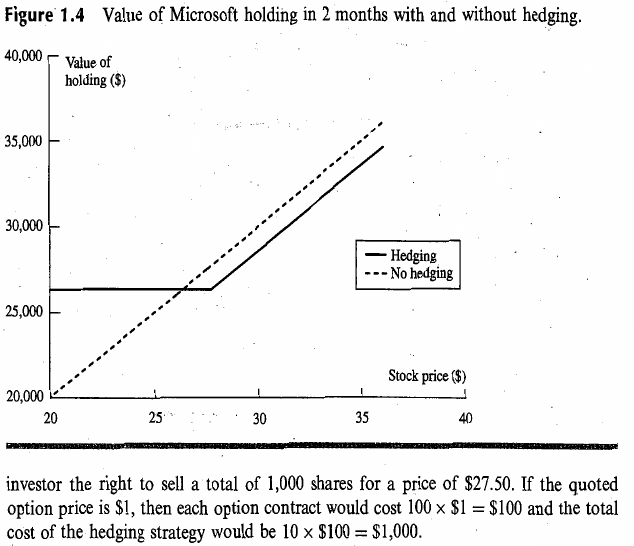
\includegraphics{hedge}\protect\caption{Hedging}


\end{figure}


So how much should you pay for such a right (either call or put)?
Alternatively how much can you charge if you're selling such a contract?
The basic idea in figuring out how to price such a contract is to
assume that no arbitrages exist in the market and use delta hedging
(fractional shares) to construct a perfect hedge (one that eliminates
all risk from a portfolio). Since the portfolio is riskless it must
earn interest at the risk-free rate. From this you can calculate the
value of the portfolio at expiration and work backwards to see how
much the option should have the buyer.


\subsection{Black-Scholes}

The Black-Scholes model was constructed by Fischer Black and Myron
Scholes in 1973, based on work by Robert Merton. Merton and Scholes
won the Nobel in Economics in 97 (Black was ineligible having died
in 95). It forms the basis for much more complicated investment strategies
used by hedge funds.

The Black\textendash Scholes model assumes that the market consists
of at least one risky asset, usually called the stock, and one riskless
asset, usually called the money market, cash, or bond. The assumptions
on market are
\begin{itemize}
\item There is no arbitrage opportunity (i.e., there is no way to make a
riskless profit).
\item It is possible to borrow and lend any amount, even fractional, of
cash at the riskless rate.
\item It is possible to buy and sell any amount, even fractional, of the
stock.
\item The above transactions do not incur any fees or costs (i.e., frictionless
market).
\end{itemize}
The assumptions on the assets are
\begin{itemize}
\item The rate of return on the riskless asset is constant and thus called
the risk-free interest rate.
\item The instantaneous log returns of the stock price is a geometric Brownian
motion, and we will assume its drift and volatility is constant.
\item The stock does not pay a dividend.
\end{itemize}
Per the model assumptions above, the price of the underlying asset
(typically a stock) follows a geometric Brownian motion. That is
\[
\frac{dS}{S}=\mu dt+\sigma dB
\]
We now construct a portfolio $\Pi$ consisting of some number of European
call options on the stock and some number of shares which is a perfect
hedge (riskless). First the price of the call option $V$ is a stochastic
process and clearly a function of $S_{t}$ and $t$. So by Ito's lemma
\[
dV=\left(\mu S\frac{\partial V}{\partial S}+\frac{\partial V}{\partial t}+\frac{1}{2}\sigma^{2}S^{2}\frac{\partial^{2}V}{\partial S^{2}}\right)dt+\sigma S\frac{\partial V}{\partial S}dB
\]
Now delta-hedging portfolio that turns out to be a perfect hedge is
to sell 1 option and buy $\frac{\partial V}{\partial S}$ shares of
the stock. It will become clear in a moment why this is the portfolio
that turns out to be a perfect hedge. The value of this portfolio/holdings
is 
\[
\Pi=-1\times V+\frac{\partial V}{\partial S}S
\]
Why? First note that we're on the sell side of the option. Meaning
we have sold someone else the right to sell us something, at the expiration
of the option. What happens if the price of the stock exceeds the
strike price of the option? Then it wouldn't make sense for the buyer
to sell us shares of the stock at the strike price because they would
be losing money. Alternatively if the price of the stock is below
the strike price then it does make sense for the buyer to sell us
shares of the underlying. This is the value $V$ of the option and
to us it's a loss (because end up paying above market rate for the
shares). Because we're on the sell side of the option (we sold a call
option). On the otherhand the value of our holdings in the underlying
$\left(\frac{\partial V}{\partial S}S\right)$ is a gain (since the
shares simply have their face value). 

Discretizing the differentials in$\Pi$: from $t$ to $t+\Delta t$
the net change in the value of the portfolio is
\[
\Delta\Pi=-\Delta V+\frac{\partial V}{\partial S}\Delta S
\]
Similarly discretising the process that defines $S$ and $V$ 
\begin{eqnarray*}
\Delta S & = & \mu S\Delta t+\sigma S\Delta B\\
\Delta V & = & \left(\mu S\frac{\partial V}{\partial S}+\frac{\partial V}{\partial t}+\frac{1}{2}\sigma^{2}S^{2}\frac{\partial^{2}V}{\partial S^{2}}\right)\Delta t+\sigma S\frac{\partial V}{\partial S}\Delta B
\end{eqnarray*}
Note ratios of differentials haven't been discretised because \_\_\_\_\_\_\_.
Now substituting into $\Delta\Pi$
\[
\Delta\Pi=\left(-\frac{\partial V}{\partial t}-\frac{1}{2}\sigma^{2}S^{2}\frac{\partial^{2}V}{\partial S^{2}}\right)\Delta t
\]
Note that $\Delta B$ dependence drops out. The portfolio is now riskless
(independent of the stochastic volatility in the market). Therefore
the rate of return must be the risk-free rate $r$ (otherwise there
would be arbitrage in the market because you could earn money on this
riskless portfolio at a greater rate than the risk-free rate). Hence
\[
\Delta\Pi=r\Pi\Delta t
\]
If this is unrecognizable think 
\[
\frac{d\Pi}{dt}=r\Pi
\]
i.e. continuously compounding interest. Equating the two expressions
for $\Delta\Pi$ we get 
\[
\left(-\frac{\partial V}{\partial t}-\frac{1}{2}\sigma^{2}S^{2}\frac{\partial^{2}V}{\partial S^{2}}\right)\Delta t=r\left(-V+S\frac{\partial V}{\partial S}\right)\Delta t
\]
or 
\[
\frac{\partial V}{\partial t}+\frac{1}{2}\sigma^{2}S^{2}\frac{\partial^{2}V}{\partial S^{2}}+rS\frac{\partial V}{\partial S}-rV=0
\]
the Black-Scholes equation. Solving this PDE with boundary conditions

\begin{align}V(0,t) & =0\text{ for all }t\\
V(S,t) & \rightarrow S\text{ as }S\rightarrow\infty\\
V(S,T) & =\max\left\{ S-K,0\right\} 
\end{align}

gives the value of the option for all $t\leq T$. To actually solve
recognize it as a Cauchy-Euler equation which can be transformed into
a diffusion equation with the change of variables
\begin{eqnarray*}
\tau & = & T-t\\
u & = & Ve^{r\tau}\\
x & = & \ln\left(\frac{S}{K}\right)+\left(r-\frac{1}{2}\sigma^{2}\right)\tau
\end{eqnarray*}
to produce
\[
\frac{\partial u}{\partial\tau}=\frac{1}{2}\sigma^{2}\frac{\partial^{2}u}{\partial x^{2}}
\]
with boundary condition $V\left(S,T\right)=\max\left\{ S-K,0\right\} $
becoming initial condition
\[
u\left(x,0\right)=u_{0}\left(x\right)=K\left(e^{\max\left\{ x,0\right\} }-1\right)
\]
The standard solution is by method of Green's functions
\begin{eqnarray*}
u\left(x,\tau\right) & = & \frac{1}{\sigma\sqrt{2\pi\tau}}\int_{-\infty}^{\infty}u_{0}\left(y\right)e^{-\frac{\left(x-y\right)^{2}}{2\sigma^{2}\tau}}dy\\
 & = & Ke^{x+\frac{1}{2}\sigma^{2}\tau}\Phi\left(d_{1}\right)-K\mathcal{\Phi}\left(d_{2}\right)
\end{eqnarray*}
where $\Phi$ is the CDF of a standard normal and 

\begin{align}d_{1} & =\frac{1}{\sigma\sqrt{\tau}}\left[\left(x+\frac{1}{2}\sigma^{2}\tau\right)+\frac{1}{2}\sigma^{2}\tau\right]\\
d_{2} & =\frac{1}{\sigma\sqrt{\tau}}\left[\left(x+\frac{1}{2}\sigma^{2}\tau\right)-\frac{1}{2}\sigma^{2}\tau\right]
\end{align}


\end{document}
